\section{Demo Setup}
Our demo system is implemented in Java and can be deployed on any
PC or workstation with at least 8GB of memory and running JRE 1.6.0 and above. 
A J2EE application container is also required. We use Tomcat 7.0.41.
Next we briefly describe the steps in the proposed demo.

\begin{figure}[th]
\centering
\includegraphics[scale=0.28]{screenShot1_2.eps}
\caption{Configuration of the Simulation (the purple line is  
the selected path)}
\label{fig:screen_shot1}
\end{figure}

In step 1 (Figure \ref{fig:screen_shot1}), user first picks a scene 
(e.g. exhibition hall or shopping mall) and select the number of nodes 
as well as the total duration of the simulation ($T$ in Section 
\ref{sec:approach}). Then, with the mouse, user can pick the paths 
for some or all of the objects on the map as the ground truth. 
The exact timing of the trajectory
is determined by the system using one of the predefined speed distributions.  
The total duration $T$ is useful in automatically generate paths 
for the objects whose paths were not selected by the user.

\begin{figure}[th]
\centering
\includegraphics[scale=0.5]{screenShot2_2.eps}
\caption{Induced Contact History from Running the Simulation}
\label{fig:screen_shot2}
\end{figure}

In step 2, when ``Generate'' button is pressed, 
the system will simulate the movements of the objects and 
compute the contact history. This history is displayed to the user for 
verification (Figure \ref{fig:screen_shot2}).  
Now the user can press ``Infer'' button to start the inference
algorithm.

\begin{figure}[th]
\centering
\includegraphics[scale=0.25]{screenShot3_2.eps}
\caption{Inference Results Playback}
\label{fig:screen_shot3}
\end{figure}

Finally in step 3 (Figure \ref{fig:screen_shot3}), use can select a node id
to compared the ground truth trajectory with the inferred trajectory side by
side by pressing the ``Play'' button and see the animation.

%Our system provides data sets with variance configuration. Before every thing starts, you must select one of them. First, select a data set (map) using the droplist on the right side. The map you select will be showed on the left side. Next, fill in some essential parameters for the simulation. eg. number of people,duration. The configuration for people is provided, but you can custem made one or two of them by selecting the path (the purple line in Figure~\ref{fig:screen_shot1})they may follow and the distribution. Figure~\ref{fig:screen_shot1} show a snapshot of this step.
%
%Then, you come the step shows in Figure~\ref{fig:screen_shot2}. Click the "Run" button to start the simulation. You can see the contact generation log on the left textarea. 
%Those two steps above is doing preparation for the main part. Now, we are going to run these contacts. Click the "Infer" button in Figure~\ref{fig:screen_shot3} to start our inference computation. After a reansonable computation delay, you can get the inference result. Select a person you want to see, and click "Play" button. Then, the person's historical location will be showed on the map time by time. You can view this on the left side. Also, a corresponding background truth will also be provied for comparaison.


